\documentclass[tikz,border=4pt]{standalone}
\usepackage{amsmath,amssymb}

\usetikzlibrary{arrows.meta,positioning,automata,shapes,shapes.misc,calc,decorations.pathmorphing,decorations.markings,angles,quotes,patterns,mindmap,matrix,knots,hobby,trees}
\tikzset{->-/.style={decoration={markings, mark=at position 0.5 with {\arrow{Stealth}}}, postaction={decorate}}}
\begin{document}
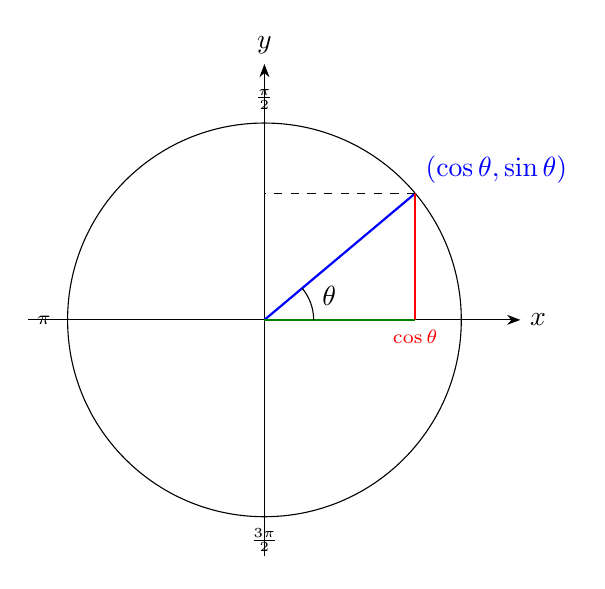
\begin{tikzpicture}[scale=2.5, >=Stealth]
\draw[->] (-1.2,0) -- (1.3,0) node[right] {$x$};
\draw[->] (0,-1.2) -- (0,1.3) node[above] {$y$};
\draw (0,0) circle (1);
\draw[thick, blue] (0,0) -- (40:1) node[above right] {$(\cos\theta, \sin\theta)$};
\draw[thick, red] (40:1) -- ({cos(40)},0) node[below, pos=1] {\scriptsize $\cos\theta$};
\draw[thick, green!50!black] ({cos(40)},0) -- (0,0);
\draw (0.25,0) arc (0:40:0.25); \node at (20:0.35) {$\theta$};
\foreach \a/\l in {90/{\frac{\pi}{2}}, 180/\pi, 270/{\frac{3\pi}{2}}} \node[font=\scriptsize] at (\a:1.12) {$\l$};
\draw[dashed] (40:1) -- (0,{sin(40)});
\end{tikzpicture}
\end{document}
